\begin{wrapfigure}{l}{0pt}
  \centering
  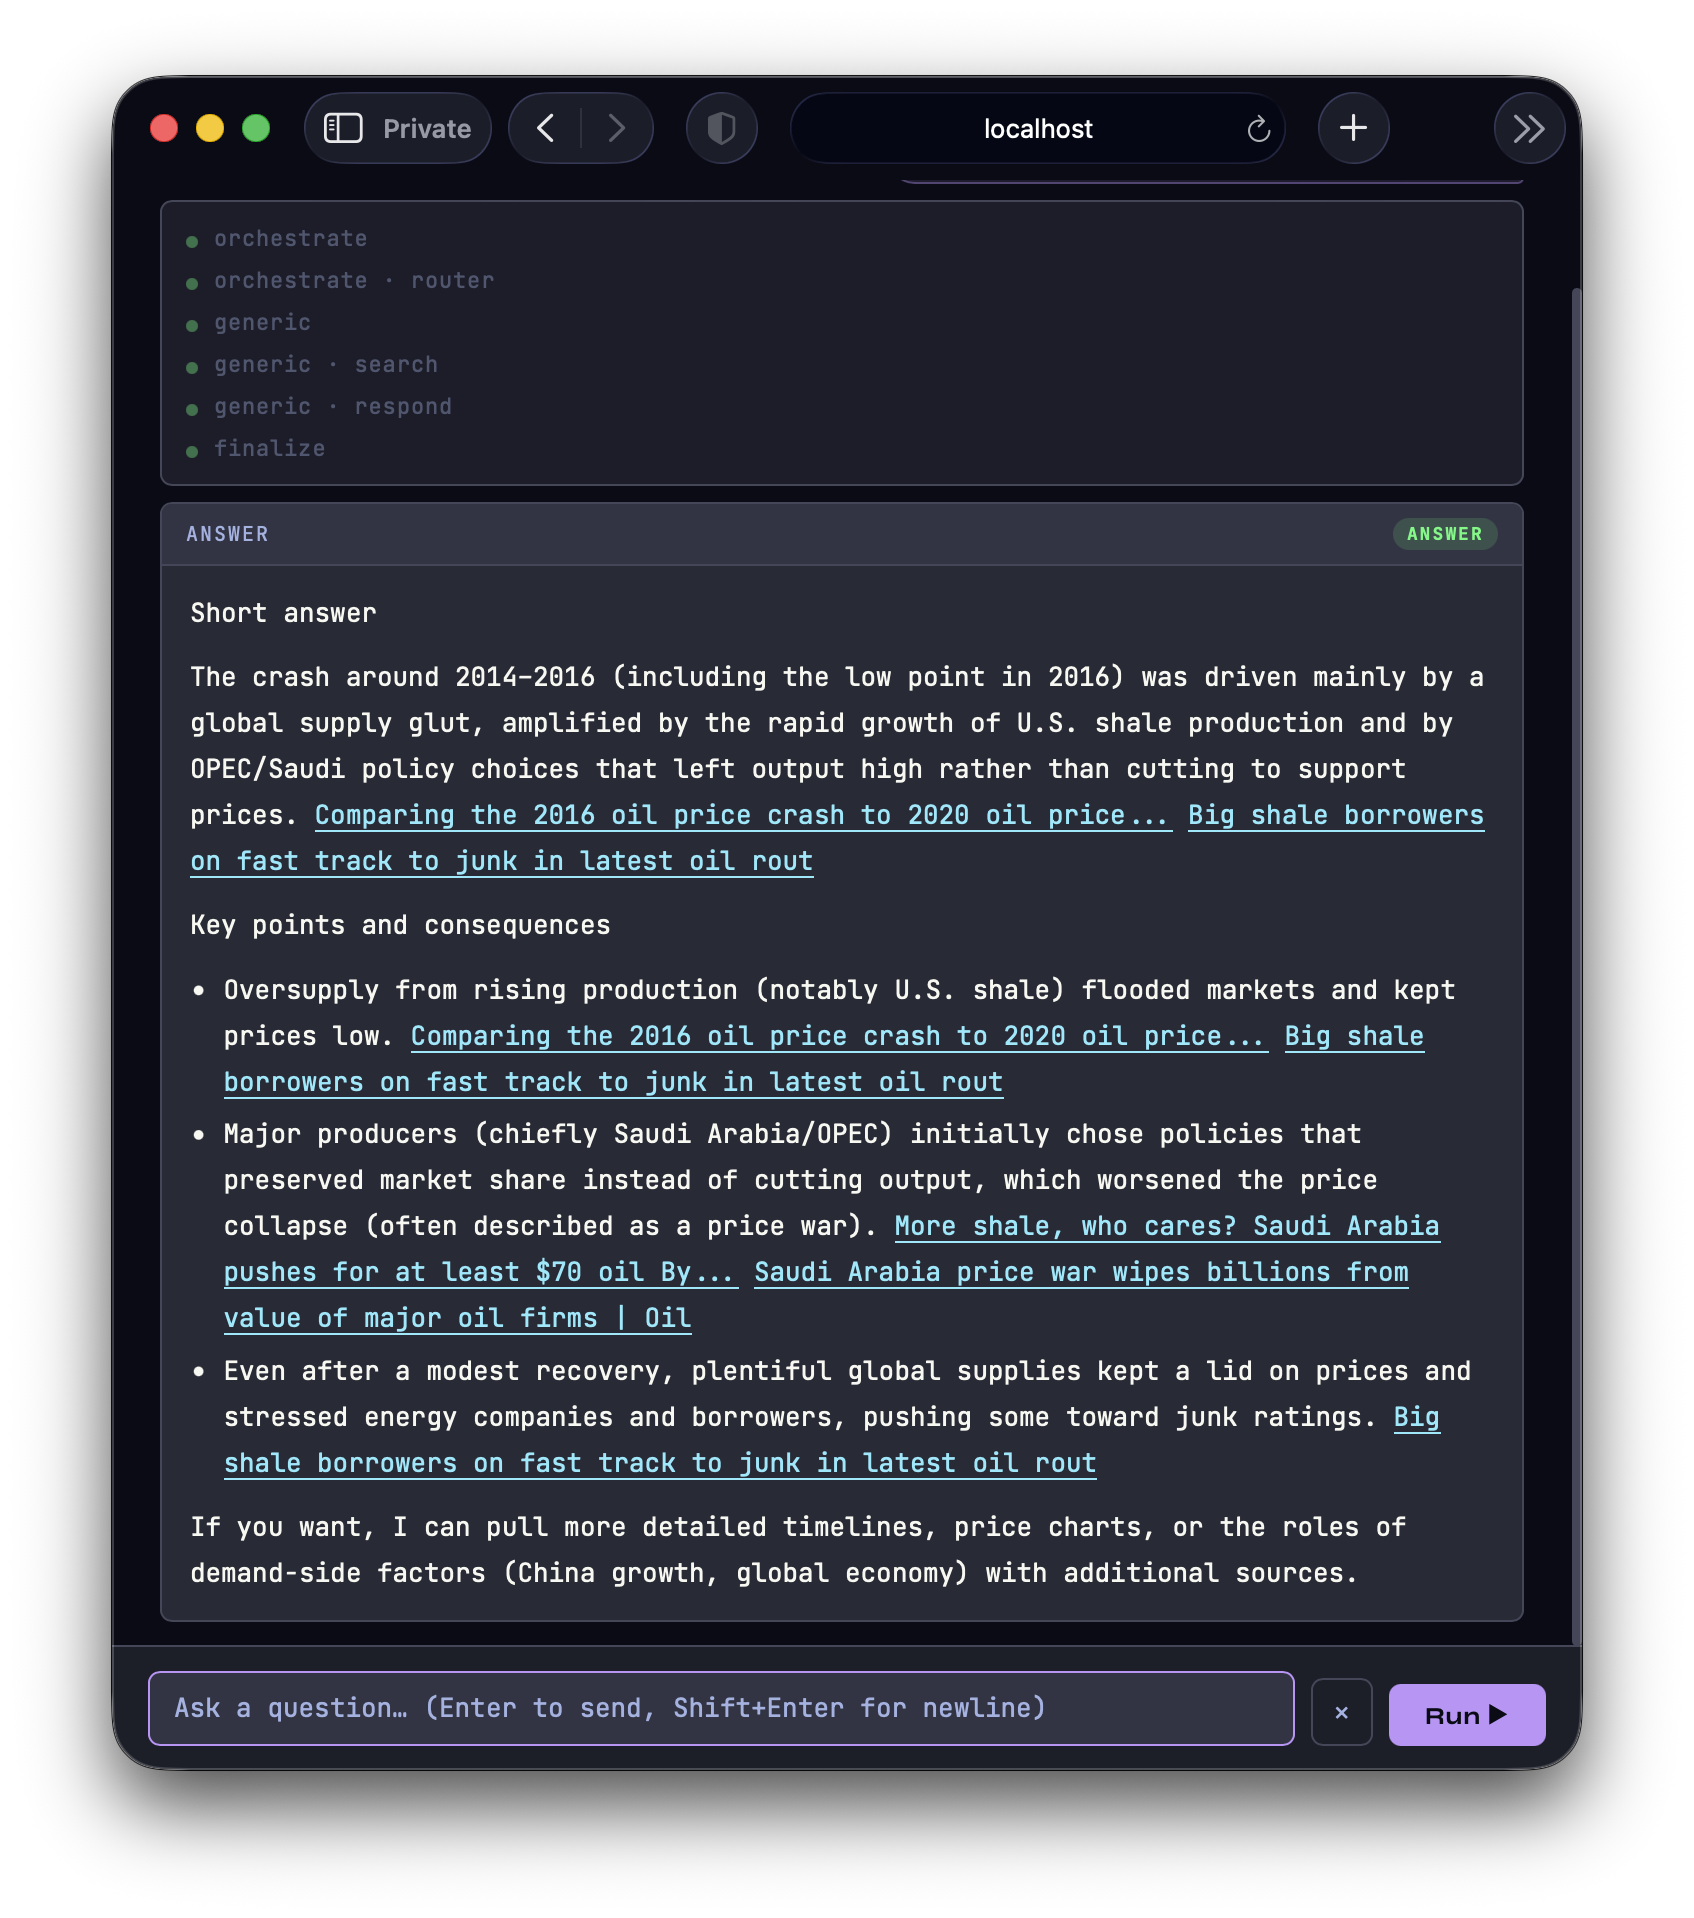
\includegraphics[width=0.4\textwidth]{graphics/ui-what-caused-the-2016-oil-price-crash.png}
  \caption{UI Screenshot}
\end{wrapfigure}

The primary goal was to identify and explain the confluence of factors responsible for the sharp decline in global oil prices around 2016. The agent utilized a multi-step process involving information retrieval, causal relationship mapping, and synthesis across various economic reports.

\subsect{Step 1: Information Retrieval \& Scope Definition}
The query was broken down into key search concepts: (a) timeline/event ("2016 oil price crash"), (b) mechanisms of collapse (causes), and (c) major industry players (OPEC, Saudi Arabia, U.S. Shale). The agent successfully retrieved several articles establishing the context:
\begin{itemize}
  \item \textbf{Timeline Confirmation:} Sources confirmed that the collapse was a protracted event spanning 2014–2016 [Nairametrics].
  \item \textbf{Key Players/Factors:} Results highlighted the roles of U.S. shale oversupply, OPEC decisions, and Saudi policy (price war).
\end{itemize}

\subsect{Step 2: Causal Factor Analysis \& Mapping}
The agent did not simply list facts; it analyzed *how* these factors interacted to create a collapse. Two primary causal dimensions were mapped:

\subsubsect{A) Supply-Side Pressure (Oversupply)}
Multiple sources pointed to an unchecked increase in global supply as the fundamental trigger. The rapid development and output of U.S. shale production played a critical role, overwhelming market capacity and keeping prices suppressed [Nairametrics]. This established the base condition: persistent oversupply.

\subsubsect{B) Policy Failure (Producer Behavior)}
The agent identified that the response from major producers was exacerbating, rather than mitigating, the crisis. Key findings showed:
\begin{itemize}
\item Saudi Arabia's attempts to maintain market value by refusing deep cuts [Investing].
\item The resulting "price war" among major firms, which wiped out billions in market value [The Guardian].
\end{itemize}
This established that the policy decision (maintaining output share vs. cutting supply) actively worsened the price decline.

\subsect{Step 3: Synthesis and Structuring the Answer}
Finally, the agent synthesized these two dimensions into a cohesive narrative structure suitable for a report summary, defining the collapse as the interaction of market oversupply $\textbf{plus}$ poor policy coordination. The final answer clearly delineates the key points:

\begin{enumerate}
\item \textbf{Root Cause:} Global supply glut (Shale).
\item \textbf{Amplifying Factor:} Producer decisions that prevented necessary output cuts (Policy/Price War).
\item \textbf{Consequence:} Prices remained capped despite recovery attempts, posing financial risks to energy sectors and borrowers.
\end{enumerate}

This systematic approach ensured the answer was not merely a collection of facts but a detailed explanation of the complex economic mechanism that led to the 2016 oil price crash.
